%
% Ce document est écrit au format UTF-8.
% Il est adapté depuis http://www.sigchi.org/publications/chipubform.
%
\documentclass{ihm}

% Décommentez cette ligne pour remettre les numéros de page.
% \pagenumbering{arabic}

\usepackage{listings}

% Quelques packages indispensables.
\usepackage{balance}
\usepackage{graphics}
\usepackage{times}
\usepackage{url}

% Style pour les URLs
\makeatletter
\def\url@leostyle{%
  \@ifundefined{selectfont}{\def\UrlFont{\sf}}{\def\UrlFont{\small\bf\ttfamily}}}
\makeatother
\urlstyle{leo}


% Ne pas modifier
\def\pprw{21cm}
\def\pprh{29.7cm}
\special{papersize=\pprw,\pprh}
\setlength{\paperwidth}{\pprw}
\setlength{\paperheight}{\pprh}
\setlength{\pdfpagewidth}{\pprw}
\setlength{\pdfpageheight}{\pprh}

% Hyperref doit être le dernier package à inclure.
% N'oubliez pas de renseigner les informations qui se trouvent ici.
\usepackage[pdftex]{hyperref}
\hypersetup{
pdftitle={Format des publications finales pour IHM'13},
pdfauthor={LaTeX},
pdfkeywords={format, instructions, qualité, actes de conférence},
bookmarksnumbered,
pdfstartview={FitH},
colorlinks,
citecolor=black,
filecolor=black,
linkcolor=black,
urlcolor=black,
breaklinks=true,
}

% Utilisez \tabhead{} pour les en-têtes de tableaux.
\newcommand\tabhead[1]{\small\textbf{#1}}

% Pour les listings dans LE langage
\renewcommand\lstlistingname{Définition}
\renewcommand\lstlistlistingname{Définitions}
\def\lstlistingautorefname{Définition }

% Début du document
\begin{document}

\lstdefinelanguage{myl}
{morekeywords={
Interactor,
Components,
If,
In,
Out,
Interface,
Behavior,
Init,
Always,
When,
State},
sensitive=false,
morecomment=[l]{//},
morecomment=[s]{/*}{*/},
morestring=[b]",
}

\lstset{
    language=myl,
    basicstyle=\small,            % print whole listing small
    keywordstyle=\color{black}\bf,% underlined bold black keywords
    tabsize=2,                    % sets default tabsize to 2 spaces
    captionpos =b                 % sets the caption-position to bottom
    keepspaces = true             % keeps spaces in text
    % identifierstyle=,           % nothing happens
    commentstyle=\textit,         % white comments
    stringstyle=\ttfamily,        % typewriter type for strings
    showstringspaces=false,       % no special string spaces
    columns=flexible,             % colonnes "flexibles"
    basewidth={0.45em},           % dimension des colonnes
    fontadjust=true,              % pour ajuster les polices
    breaklines=true}              % pour le retour à la ligne dans les colonnes


\title{Un langage formalisable pour la définition d'applications interactives
  embarquées et critiques}

\numberofauthors{3}
\author{
  \alignauthor Vincent Lecrubier\\
    \affaddr{ONERA}\\
    \affaddr{2 Avenue Edouard Belin}\\
    \affaddr{31400, Toulouse, France}\\
    \email{Vincent.Lecrubier@onera.fr}
  \alignauthor Bruno d'Ausbourg\\
    \affaddr{ONERA}\\
    \affaddr{2 Avenue Edouard Belin}\\
    \affaddr{31400, Toulouse, France}\\
    \email{Bruno.d.Ausbourg@onera.fr}
  \alignauthor Yamine Aït-Ameur\\
    \affaddr{INPT/ENSEEIHT}\\
    \affaddr{2 rue Charles Camichel}\\
    \affaddr{31000, Toulouse, France}\\
    \email{yamine@enseeiht.fr}
}

\maketitle

\begin{abstract}
Cet article décrit et utilise le format de mise en page à respecter pour les
soumissions à IHM'13. Après acceptation, ces soumissions seront publiées dans
les actes d'IHM'13, ainsi que sur l'ACM Digital Library, sauf les communications
informelles qui seront publiées dans un volume annexe séparé. Comme certains
détails ont changé par rapport aux années précédentes, nous vous prions de bien
lire ce document même si vous avez déjà soumis à IHM auparavant.
\end{abstract}

\keywords{
	Format; instructions; qualité; actes de conférence; les mots-clés doivent
	être séparés par des points-virgules.
}

\category{H.5.m.}{Information Interfaces and Presentation (e.g. HCI)}{Miscellaneous}.
Voir \url{http://www.acm.org/about/class/1998/} pour la liste complète des catégories ACM.

\section{Introduction}

Méthodes  et  techniques de  descriptions  formelles  ont été,  depuis
longtemps, appliquées au  domaine des des systèmes  critiques pour des
besoins  de  sûreté.  C'est   particulièrement  le  cas  des  systèmes
aéronautiques  dont le  fonctionnement peut  mettre en  jeu la  vie de
passagers.   De  nombreux travaux  de  recherche  se sont  attachés  à
élaborer et proposer des moyens pour concevoir, programmer et vérifier
les   fonctionnalités    de   systèmes   critiques    en   particulier
aéronautiques.   Ces  systèmes et  les  processus  qui encadrent  leur
développement sont par ailleurs  l'objet d'étapes de certification qui
établissent que  le produit  et le  développement qui  a conduit  à le
construire  sont  en conformité  avec  des  standards établissant  des
règles précises les définissant, tels  la DO178C \cite{DO178C} pour le
logiciel aéronautique embarqué.

Les systèmes  d'interaction homme-machine (IHM) n'ont  bénéficié ni de
la  même attention  ni  du  même effort  de  recherche.  Pourtant  des
systèmes d'interaction  mettant en oeuvre des  capacités électroniques
et numériques hautement sophistiquées ont fait leur apparition au sein
de cockpits d'avions de nouvelle  génération.  Ces systèmes se fondent
sur  des  logiciels à  la  fois  volumineux  et complexes  et  doivent
répondre  à des  contraintes  sévères en  matière d'utilisabilité,  de
sécurité  ou  de   sûreté.   Ces  logiciels  mettent   en  oeuvre  des
applications dont le comportement, compte tenu de leur criticité, doit
se  conformer avec  un  niveau très  élevé d'assurance  à  ce qui  est
attendu  du système.  En effet  une  erreur dans  l'un des  composants
d'interaction logiciels peut conduire à  une erreur humaine ou système
dont les effets peuvent se révéler catastrophiques.

Le récent rapport du Bureau  d'Enquêtes et d'Analyses \cite{BEA12} sur
le crash  de l'Airbus A330  d'Air France  lors du vol  AF447 Rio-Paris
pointe  un réel  dysfonctionnement du  système d'interaction,  et plus
particulièrement du  directeur de  vol, ayant affiché  des indications
qui n'auraient pas dû l'être et ayant ainsi conduit le pilote à cabrer
son appareil alors que ce dernier était déjà en train de décrocher.

Le  coeur du  problème réside  essentiellement  dans le  fait que  les
processus  standards  de   développement  des  systèmes  aéronautiques
critiques se fondent la plupart du  temps sur des cycles linéaires (du
type des  cycles en V  ou de ses variantes)  qui s'avèrent peu  ou mal
adaptés   à  la   conception   et  au   développement  des   logiciels
d'interaction qui  requièrent des  cycles d'itérations  impliquant les
usagers et mêlant opérations de test  et phases de conception dans les
processus mis en oeuvre. Une autre difficulté, propre au développement
des  systèmes  d'interaction,  est  imputable à  la  multiplicité  des
communautés techniques  et scientifiques intervenant dans  le champ de
la définition des systèmes d'IHM.  Manquent à ces communautés diverses
un  langage et  des notations  qui  soient, sinon  communes, du  moins
intelligibles par toutes. Dès lors le traitement de la sûreté et de la
sécurité  de ces  systèmes  d'interaction critiques  ne  fait appel  à
aucune  méthode ni  aucun outil  spécifiques.  Dans  ce contexte,  les
processus de validation  de ces systèmes demeurent pauvres  car ils se
limitent pratiquement à des phases  intensives de test et d'évaluation
en fin  de processus de développement,  qui plus est sans  disposer de
réelle  référence, en  particulier  formelle, vis  à  vis de  laquelle
confronter le système développé.

Ce  papier  suggère d'introduire  cette  référence  formelle lors  des
étapes  amont  des  processus  de  développement  des  systèmes  d'IHM
critiques  en  proposant un  langage,  formalisable,  qui permette  la
description des  applications interactives,  tant du  point de  vue de
leur présentation que de leur  comportement, ainsi que l'expression d'
exigences des concepteurs concernant  l'interaction encodée au sein de
ces  applications.   Ce langage  veut  être  suffisamment abstrait  et
convivial pour être compris et utilisables par tous les participants à
la conception  et au développement  de l'IHM. Il veut  également être,
sinon formel,  du moins  formalisable de telle  sorte que  qu'un texte
rédigé  dans   ce  langage  puisse   être  soumis  à   des  opérations
automatiques  ou  semi-automatiques  de vérifications  et  de  preuves
formelles, de génération de tests  pertinents du système à développer,
et de génération de code plus  sûr. De manière à accroître l'assurance
que le logiciel développé se comporte bien comme prévu.

\section{Travaux connexes}
\label{sec:travaux}

La formalisation des systèmes d'interaction a pourtant fait l'objet de
travaux  importants  lors  de  ces dernières  années:  bon  nombre  de
modèles, de langages ou de méthodes  formels ont vu le jour pour aider
à spécifier, concevoir, vérifier et implanter ces systèmes.

Une première classe  de modèles basés sur les  systèmes de transitions
et plus particulièrement sur  les extensions d'automates d'états finis
et de  réseaux de Petri ont  utilisé les automates d'états  finis pour
décrire  des   comportements  interactifs  de  base.    De  manière  à
circonvenir  les  problèmes liés  à  l'explosion  combinatoire de  ces
modèles  de  nombreuses extensions  ont  été  proposées. Les  machines
d'états  hiérarchiques  ou  les statecharts  décrivent  des  automates
composables  facilitant  la  spécification de  systèmes  complexes  et
permettant la réutilisation  des modèles. Les automates  à états finis
peuvent  être  utilisés  dans   le  cadre  d'outils  de  programmation
\cite{Blanch02,Blanch06}   ou  peuvent   être   associés  à   d'autres
formalismes      pour      décrire       d'autres      aspects      de
l'interaction. En \cite{Jacob99} les  automates modélisent les apsects
de l'interaction liés à des entrées  discrètes tandis que les flots de
données représentent les entrées continues. 

Le modèle  de capteurs formels  \cite{Accot97} utilise les  réseaux de
Petri de haut niveau  \cite{Jensen95} pour décrire les transdormations
successives  d''événements  d'entrée. Les  réseaux  de  Petri ont  été
utilisés  par  plusieurs  méthodes  et  techniques  pour  décrire  les
systèmes  d'IHM.  Le  formalisme  ICO \cite{palanque93,palanque97}  se
fonde sur  une approche orientée  objet pour modéliser  les composants
statiques d'un système d'interaction et  sur les réseaux de Petri pour
en  décrire  la  dynamicité  :  PetShop  \cite{Bastide02,Schyn03}  est
l'outil basé sur ICO.

D'autres descriptions  formelles des  systèmes interactifs  se fondent
sur la  notion d'interacteurs.  Les interacteurs  peuvent se concevoir
comme  des  entités  autonomes et  communicantes  interagissant  entre
elles, de  manière interne au système  d'interaction, ou interagissant
de façon  externe avec le système  interfacé ou l'usager par  le biais
d'événements (ou de stimuli). Les deux premiers modèles d'interacteurs
développés le  furent dans le  cadre du  projet AMODEUS. Le  modèle de
York \cite{york93}  fournit un cadre  pour la description  de systèmes
d'interaction à l'aide de notations  orientées modèles telles que Z ou
VDM.   Le  modèle  du  CNUCE  \cite{Paterno92}  utilise  quant  à  lui
LOTOS. Des interacteurs formels ont également été décrits en utilisant
le  langage synchrone  Lustre :  \cite{nousdsvis96} montre  comment de
tels interacteurs peuvent être dérivés d'une description informelle du
système d'interaction. Ces interacteurs  formels peuvent être composés
pour constituer  un modèle  formel de l'IHM  et peuvent  être utilisés
pour vérifier le système conçu  ou générer des tests \cite{dsvis98} et
pour, plus  généralement, valider  le système  d'interaction développé
\cite{ausbourg98}. 

\cite{yamine98a,yamine98b} introduisent  une approche  modulaire basée
sur  l'usage  de  la  méthode  B.   Les  spécifications  d'un  système
interactif opérationnel  y sont formalisées en  assurant qu'un certain
nombre   de   propriétés   ergonomiques   sont   préservées   par   le
système. Diverses formes d'interaction  ont ainsi été formalisées dans
le cadre  de ces travaux  en permettant la vérification  de nombreuses
propriétés de  ces systèmes telles leur  observabilité, leur honnêteté
ou leur robustesse.  Le travail  présenté en \cite{yamine00} montre la
description  et la  preuve, à  l'aide de  B, de  toutes les  étapes de
raffinement  d'un  modèle  abstrait  de  système  jusqu'à  son  codage
concret.

Le  grand  mérite  de  ces  travaux est  ainsi  d'avoir  démontré  que
l'interaction peut être formalisée et est donc formalisable. Toutefois
ces  approches   construisent  leurs  modèles  directement   dans  les
formalismes  cibles.   Cela  nécessite  donc une  bonne  maîtrise  des
notations offertes  par ces  formalismes. C'est  sans doute  la raison
pour laquelle ces tentatives n'ont  pas vraiment abouti dans la mesure
où  la communauté  des  concepteurs et  développeurs  ne s'est  jamais
approprié les techniques qu'elles proposaient.

En  revanche  beaucoup  de  travaux  de recherche  ont  porté  sur  la
définition et les transformations de modèles de tâches avec l'objectif
général,  partant   d'un  modèle  abstrait  des   tâches  assignées  à
l'utilisateur, d'en dériver des  modèles d'IHM.  Ces approches mettent
ainsi  l'accent  sur  la  définition  des tâches  plutôt  que  sur  la
conception de  l'IHM proprement  dite.  Même lorsqu'ils  s'attachent à
définir   des   langages   d'interfaces   abstraites,   comme   USIXML
\cite{UsiXML},  ces derniers  restent  profondément  orientés sur  les
tâches de l'usager plutôt que sur les détails d'interaction.

Il semble donc utile de proposer  un langage de définition de systèmes
d'interaction  utilisable et  disposant  de la  capacité d'offrir  les
mêmes services que les formalismes précédemment expérimentés.

\section{Objectifs d'un langage de définition d'IHM} 

Constituer  un  langage  commun,  pivot,   qui  permette  à  tous  les
protagonistes  de  la  conception  et du  développement  d'un  système
interactif, designers,  programmeurs, ergonomes,  ingénieurs systèmes,
ainsi  que  spécialistes  des   facteurs  humains  ou  d'architectures
logicielles de collaborer  à la définition d'un même  système, tel est
sans  doute l'un  des premiers  objectifs d'un  langage de  définition
d'IHM.

Offrir  un langage  d'abstraction  de l'IHM  permet  au concepteur  de
s'adapter aux évolutions permanentes des technologies dans le monde de
l'IHM.   En  effet  celui-ci  vit actuellement  une  phase  de  grande
diversification  au  point  que   de  nombreux  et  nouveaux  horizons
s'ouvrent aujourd'hui devant les concepteurs des systèmes interactifs.
Cet enrichissement  des outils et  des dispositifs de  l'interaction a
cependant son revers.   Celui de déplacer le centre  d'attention et de
réflexion du  concepteur du problème conceptuel  d'interaction qui lui
est posé à  celui de l'implantation concrète à l'aide  des moyens dont
il  dispose  nouvellement. Passant  trop  rapidement  du besoin  à  la
solution et privilégiant  la mise en oeuvre du moyen  sur l'analyse de
la fin, le  concepteur risque alors de définir un  système inadapté au
besoin de  son utilisateur.  L'abstraction  fournie par un  langage de
définition conçu à cet effet peut lui fournir le moyen de se recentrer
efficacement sur les aspects conceptuels  de l'IHM et lui permettre de
se poser les bonnes questions à propos de l'interaction envisagée.

Un dernier  service attendu de ce  langage de définition d'IHM  est de
permettre la vérification de proprietés ou exigences de sûreté le plus
en amont possible  du cycle de développement. A  l'heure actuelle, ces
vérifications  ne  peuvent  être  opérées dans  le  meilleur  des  cas
qu'après une certaine concrétisation du  concept d'IHM et dans le pire
des cas qu'après implantation complète  de l'IHM lors des campagnes de
tests.  Des erreurs,  dont certaines peuvent s'avérer  très graves, ne
sont susceptibles d'être  détectées que lors de  la validation finale,
obligeant  alors à  réitérer  un  nouveau cycle  de  conception et  de
développement. Être sinon  formel du moins formalisable  de manière à
permettre la vérification  formelle de ces proprietés  et exigences de
sûreté dès les premières phases  de conception du système, quand celui
ci  est encore  abstrait,  constitue un  premier  objectif assigné  au
langage de définition d'IHM ciblé.

\section{$L$ langage de définition d'IHM} 

\subsection{Une application jouet}

\begin{figure}[t!] 
\begin{center}
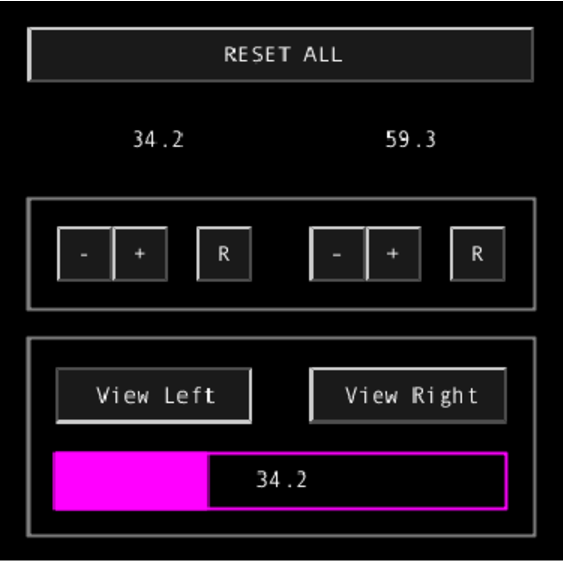
\includegraphics [scale = 0.7]{appli}
\end{center}
\caption{Une application interactive jouet}
\label{fig:appli} 
\end{figure}

La Figure  \ref{fig:appli} illustre  une application  interactive très
simple  dont la  définition abstraite  dans le  langage $L$  peut être
trouvée dans  les tableaux de  textes qui suivent.   Cette application
permet de contrôler deux valeurs réelles  à l'aide de deux panneaux de
boutons  \texttt{-,+}  et   \texttt{R}  permettant  d'incrémenter,  de
décrémenter  ou  de  remettre  à  zéro  chacune  d'elles.   Un  bouton
\texttt{Reset All}  permet de les remettre  toutes les deux à  zéro en
même temps. La visualisation de ces valeurs est réalisée sous forme de
labels exprimant leur  valeur numérique et à  travers deux dispositifs
de présentation analogiques de  valeurs réelles représentées comme des
jauges.  L'utilisateur sélectionne la jauge à afficher en agissant sur
les boutons de sélection \texttt{View Left} et \texttt{View Right}.

\subsection{Sa définition en $L$}

Le langage $L$  proposé s'articule autour de  la notion d'interacteur.
Les  interacteurs   peuvent  se   composer  pour  définir   un  nouvel
interacteur.   Un   interacteur  peut   donc  être   composé  d'autres
interacteurs qui  sont ses sous-interacteurs. Ainsi,  une IHM complète
sera représentée sous la forme d'un interacteur racine, composé de ses
sous interacteurs (fenêtres, contrôles, sons \ldots). 

Le langage cherche à permettre  la description des aspects conceptuels
et abstraits de l'IHM sans avoir  à se préoccuper de leur implantation
concrète et réelle.  Ainsi différents  types d'entités peuvent se voir
abstraits sous un même concept, ce qui simplifie grandement le langage
et son utilisation. Par exemple, les  boutons bien connus à deux états
(ToggleButton) et les cases à  cocher (CheckBox) ont une même fonction
: permettre à  l'utilisateur de communiquer une valeur  booléenne à la
machine : le concept d'entrée booléenne les représente dans le langage
à l'aide du type prédéfini \lstinline$BooleanInput$.  

Beaucoup d'éléments d'IHM sont ainsi  abstraits au sein de différentes
catégories  représentant   les  briques  de  bases   de  l'interaction
homme-machine. Les types d'interacteurs de  base du langage sont ainsi
en nombre réduit tout en permettant de prendre en compte l'intégralité
des interactions homme-machine. On trouvera  des entrées et sorties de
textes, réels,  entiers, booléens,  choix de  sous ensembles  parmi un
ensemble,  ainsi  que  de  déclenchement d'événements.  La  nature  du
langage permet  de combiner ces  briques de  base afin de  définir des
interactions plus complexes.

La description en $L$ d'un interacteur comporte quatre
sections constituant la définition de cet interacteur :
\begin{itemize}
\item une section \lstinline$State$ présentant son état : celui-ci est
  constitué de la déclaration des variables d'état de l'interacteur ;
\item une section \lstinline$Components$ déclarant les
  sous-interacteurs qui composent l'interacteur ;
\item une section \lstinline$Interface$ qui décrit les données que
  l'interacteur peut recevoir en entrée ou les événements qu'il peut
  exporter en sortie ;
\item une section \lstinline$Behavior$ qui décrit le comportement de
  l'interacteur. 
\end{itemize}

\begin{lstlisting}[float=ht!,
                   mathescape,
                   caption=\'Ecran de contrôle principal,
                   label=control,
                   frame=single]
Interactor ControlScreen // La page principale
State
	real left in [0. , 100.]
	real right in [0., 100.]
Components
  NumericOutput leftValueLabel
  NumericOutput rightValueLabel
  DualControlPanel controllers
  DualGaugePanel gauges
  TriggerInput resetButton
Behavior
  Init
    left = 0.0
    right = 0.0
	Always
		gauges.leftValue = left
		gauges.rightValue = right	
		leftValueLabel.value = left
		rightValueLabel.value = right
  When controllers.incrementLeft
	left < 100 -> left = left+1 
	When controllers.decrementLeft
	left > 0 -> left = left-1
	When controllers.resetLeft 
  left = 0
	When controllers.incrementRight
	right < 100 -> right = right+1
	When controllers.decrementRight
	right > 0 -> right = right-1
	When controllers.resetRight
	right = 0
	When resetButton.triggered
	right = 0 ; left = 0
\end{lstlisting}

Le texte de la \autoref{control} présente la définition  de l'écran de
contrôle       principal       qui       constitue       l'interacteur
\lstinline$ControlScreen$  racine de  l'application étudiée.   Si l'on
observe attentivement la structure de  ce texte il apparaît que l'état
de cet interacteur  est donné par la valeur de  deux variables réelles
\lstinline$left$ et \lstinline$right$ qui  sont les données contrôlées
par l'application.

Cet interacteur  se compose  de cinq  sous-interacteurs. Trois  de ces
sous-interacteurs  sont  d'un type  prédéfini  dans  le langage.   Les
composants  \lstinline$leftValueLabel$ et  \lstinline$rightValueLabel$
sont de type \lstinline$NumericOutput$ qui abstrait tout dispositif de
présentation     d'une     valeur     numérique.      Le     composant
\lstinline$resetButton$    est   lui    aussi   du    type   prédéfini
\lstinline$TriggerInput$   qui  abstrait   tout  dispositif   d'entrée
d'événement   de   déclenchement.    En  revanche   les   interacteurs
\lstinline$controllers$ et  \lstinline$gauges$ sont  respectivement du
type       \lstinline$DualControlPanel$      décrit       dans      la
\autoref{dualcontrolpanel}   et  du   type  \lstinline$DualGaugePanel$
défini dans la \autoref{dualgaugepanel}.


\begin{lstlisting}[float=htb!,
                   mathescape,
                   caption=Panneau de contrôle,
                   label=dualcontrolpanel,
                   frame=single]
Interactor DualControlPanel
Components
	ButtonControlPanel leftController
	ButtonControlPanel rightController
Interface
	Out incrementLeft
	Out decrementLeft
	Out resetLeft
	Out incrementRight
	Out decrementRight
	Out resetRight
Behavior
	When leftController.increment incrementLeft
	When leftController.decrement decrementLeft
	When leftController.reset resetLeft
	When rightController.increment incrementRight
	When rightController.decrement decrementRight
	When rightController.reset resetRight
\end{lstlisting}


\begin{lstlisting}[float=htb!,
                   mathescape,
                   caption=Panneau de deux jauges,
                   label=dualgaugepanel,
                   frame=single]
Interactor DualGaugePanel
State
	String visibleGauge in {"LEFT", "RIGHT"}
	Number leftValue in [0. , 100.]
	Number rightValue in [0., 100.]
Components
	NumericOutput leftGauge
	NumericOutput rightGauge
	BooleanInput viewLeftGauge
	BooleanInput viewRightGauge
Behavior
  Init
    visibleGauge = ``LEFT''
	Always
		leftGauge.visible = (visibleGauge == "LEFT")
		leftGauge.value = leftValue
		viewLeftGauge.value = (visibleGauge == "LEFT")
		rightGauge.visible =  (visibleGauge == "RIGHT")
		rightGauge.value   =  rightValue
		viewRightGauge. value = (visibleGauge == "RIGHT")
	When viewLeftGauge.changed(newValue)
	(visibleGauge != "LEFT" and newValue==true) -> 
    visibleGauge = "LEFT"
	When viewRightGauge.changed(newValue)
	(visibleGauge != "RIGHT" and newValue==true) -> 
    visibleGauge = "RIGHT"
\end{lstlisting}


\begin{lstlisting}[float=htb!,
                   mathescape,
                   caption=Panneau des boutons,
                   label=buttoncontrolpanel,
                   frame=single]
Interactor ButtonControlPanel 
Interface: 
	   Out increment
	   Out decrement
	   Out reset
Components
	TriggerInput incButton
	TriggerInput decButton
	TriggerInput resetButton
Behavior
	When incButton.triggered increment
	When decButton.triggered decrement
	When resetButton.triggered reset
\end{lstlisting}

L'ensemble  de   ces  déclarations  définit  la   partie  statique  de
l'interacteur  \lstinline$ControlScreen$. La  dynamique de  l'IHM est,
elle, définie, au travers  des sections \lstinline$Behavior$ décrivant
le comportement des interacteurs. Celui-ci s'exprime comme une machine
à  états.  L'interacteur  comprendra  ainsi un  ensemble de  variables
d'état. Un ensemble de règles  définit alors l'évolution des variables
d'état   de  l'interacteur   en  fonction   de  données   perçues  par
l'interacteur ou restituées par le biais de ses sous-interacteurs. Ces
règles  d'évolution  de  l'état de  l'interacteur  revêtent  plusieurs
formes possibles. 

La sous-section \lstinline$Init$ permet  de représenter l'état initial
de l'interacteur et des  sous interacteurs. Ainsi, à l'initialisation,
les variables d'état \lstinline$left$ et \lstinline$right$ sont toutes
deux nulles.

La   sous-section  \lstinline$Always$   définit   des  invariants   de
l'application.   Elle représente  des  proprietés  qui devront  rester
satisfaites  à  tout instant  lors  de  l'exécution. Par  exemple  les
variables  d'état \lstinline$leftValue$  et \lstinline$rightValue$  de
l'interacteur  \lstinline$gauges$  devront  toujours avoir  la  valeur
respectivement    des    variables    d'état    \lstinline$left$    et
\lstinline$right$ de l'interacteur \lstinline$controlScreen$. Il en va
de même des valeurs  des deux composants \lstinline$leftValueLabel$ et
\lstinline$rightValueLabel$  qui afficheront  donc  en permanence  les
valeurs   \lstinline$left$  et   \lstinline$right$.   Ces   invariants
établissent donc  des liens permanents  entre des variables  d'état de
l'application.   Leur  formulation   très  synthétique  est  cependant
puissante.

Les sous-sections  \lstinline$When$ permettent  de définir  toutes les
transitions  d'états qui  peuvent être  déclenchées en  réponse à  des
événements  reçus.   La  clause \lstinline$When$  définit  l'événement
déclencheur.  Cette  clause  est   généralement  suivie  d'une  garde,
précédent  le   symbole  \lstinline$->$,   qui  décrit   sous  quelles
conditions  la  transition peut  être  déclenchée.   Si la  garde  est
satisfaite  alors  la transition  est  déclenchée  et le  nouvel  état
atteint  est décrit  par les  affectations opérées  sur les  variables
d'état.

Ainsi, dans  la \autoref{control} la première  clause \lstinline$When$
indique que  l'événement déclencheur  est la réception  de l'événement
\lstinline$incrementLeft$        émis         par        l'interacteur
\lstinline$controllers$  et  defini comme  signal  de  sortie dans  la
section      \lstinline$Interface$       au      sein       de      la
\autoref{dualcontrolpanel}. Lorsque cet événement se produit, la garde
\lstinline$left < 100$  est  alors  évaluée. Si  elle  est vraie,  la
transition est  déclenchée et conduit  l'interacteur à un  nouvel état
dans lequel  la valeur  \lstinline$left$ est incrémentée  d'une unité.
Les autres définitions adoptent une structure, imposée par le langage,
équivalente à celle de la \autoref{control}. Elles appellent cependant
un certain nombre de remarques ponctuelles.


\subsection{Quelques remarques complémentaires}
\label{sec:remarques}

La  \autoref{buttoncontrolpanel}  du  type d'interacteur  composé  des
trois  boutons \texttt{-,+,R}  apparaît comme  triviale. Elle  définit
simplement trois dispositifs  déclencheurs \lstinline$TriggerInput$ et
trois événements  de sortie en \lstinline$Interface$.   Ces événements
sont  émis lorsque  l'un des  dispositifs déclencheurs  est déclenché.
Cette  définition est  donc relativement  abstraite.  Les  dispositifs
déclencheurs  peuvent être  implantés  par de  nombreux et  différents
types de widgets proposés par  diverses Toolkits. La conception en $L$
ne  s'attache  pas  à  cela  mais simplement  à  décrire  comment  les
événements  pourront   être  déclenchés   à  partir   des  dispositifs
déclencheurs. Cette définition comporte ainsi  peu de choses. Mais, du
point  de  vue de  l'interaction  et  de  son analyse,  elle  comporte
l'essentiel.

La \autoref{dualcontrolpanel}  n'offre d'autre intérêt que  de définir
l'association  de   deux  interacteurs  \lstinline$ButtonControlPanel$
décrit dans la \autoref{buttoncontrolpanel}.  Cet interacteur ne fait,
au  fond, que  relayer les  événements que  lui transmettent  ses deux
sous-interacteurs.   Ce   schéma  de  composition   particulier,  mais
fréquent en conception d'IHM,  devrait ultérieurement être directement
exprimé par  un opérateur  du langage  décrivant ce  multiplexage sans
qu'il soit nécessaire  pour le concepteur de  définir explicitement un
type d'interacteur pour cela.

La  \autoref{dualgaugepanel}  décrit   l'interacteur  formé  des  deux
jauges. Ces  dernières sont  définies comme  des interacteurs  de type
\lstinline$NumericOutput$.   Il  s'agit  donc du  même  type  abstrait
utilisé   pour   définir   les  dispositifs   de   sortie   numériques
\lstinline$leftValueLabel$  et   \lstinline$rightValueLabel$  dans  la
\autoref{control}. A cette même  abstraction la figure \ref{fig:appli}
montre qu'il correspond deux  concrétisations différentes : des labels
numériques  dans le  premier cas  et  des jauges  analogiques dans  le
second cas. En  $L$ ces deux dispositifs sont abstraits  en un seul et
même type d'interacteur. 

Enfin cette \autoref{dualgaugepanel} montre que des événements peuvent
\emph{embarquer}   avec   eux   des    objets   exprimés   comme   des
paramètres. Ainsi le type  de base prédéfini \lstinline$BooleanInput$,
comme  d'autres   types  de  base,  comporte   implicitement  dans  sa
définition  en  $L$  un attribut  \lstinline$changed$.   Cet  attribut
définit l'événement signalant que le dispositif d'entrée auquel il est
attaché a été  modifié et qu'une nouvelle valeur a  été entrée.  Cette
nouvelle  valeur est  associée à  l'événement.  Ainsi  la construction
syntaxique \lstinline$changed(newValue)$ exprime donc que la valeur de
l'interacteur auquel \lstinline$changed$ est attaché a été modifiée et
que la nouvelle valeur est portée par \lstinline$newValue$.

\section{Exploiter une définition d'application $L$}
\label{sec:verif}

\subsection{Vérification.}
Le  langage  $L$  permet  de  décrire  abstraitement  une  application
interactive comme  l'association de composants dont  chacun est défini
par   une  machine   d'états   finis.  Le   comportement  attendu   de
l'application peut être exprimé comme un ensemble de propriétés que le
système final  doit satisfaire.  Ces propriétés  peuvent préalablement
être vérifiées sur un modèle formel de cette application. Il faut pour
cela disposer d'un modèle formel de l'application et d'autre part d'un
modèle des propriétés vérifiées.

Le  langage  $L$ habille  un  certain  nombre d'attributs  sémantiques
propres à ceux  mis en oeuvre dans les langages  formels.  On retrouve
explicitement dans $L$ les notions d'états, de transitions, de gardes,
d'événements et de modularité. C'est pourquoi il est relativement aisé
de traduire  mécaniquement des textes  en $L$ en  notations formelles.
Promela \cite{Spin} est le langage permettant de rapidement formaliser
une  définition en  $L$. Promela  est  un langage  de modélisation  de
processus dont l'objectif  est de permettre de vérifier  la logique de
systèmes parallèles. Or  une application interactive peut  tout à fait
être  considérée  comme un  système  asynchrone  composé de  processus
parallèles (les interacteurs) et communiquant (données et événements).

En disposant d'un modèle Promela de l'application interactive, l'outil
Spin  peut  vérifier la  correction  de  ce  modèle en  réalisant  des
simulations itératives  ou aléatoires de l'exécution  de l'application
modélisée, ou  en générant un  programme C réalisant  une vérification
rapide et exhaustive de tout l'espace d'états de l'application. Durant
ces  simulations  ou  ces  vérifications  Spin  vérifie  l'absence  de
blocages. La vérification peut également être utilisée pour prouver la
correction  d'invariants du  système  ou  pour détecter  d'éventuelles
boucles de non  progression. Spin permet également  la vérification de
contraintes temporelles formulées en logique temporelle linéaire. 

Les exigences  ou propriétés  attendues du  système peuvent  donc être
formulées en logique temporelle linéaire pour être alors vérifiées sur
le modèle de l'application formalisée en Promela.

Ainsi, en reprenant la définition de l'application illustrée en figure
\ref{fig:appli}, il est possible de montrer sur son modèle Promela que
les formules
\begin{align*}
[](&(rightGauge.value=right)\; \wedge \\
&(leftGauge.value=left))
\end{align*}
et 
\begin{align*}
[]&(resetButton.triggered -> \\
&<> (left=0 \wedge right=0))
\end{align*} 
sont toujours satisfaites.  La première formule exprime que, dans tous
les états de l'application, la valeur reflétée par les deux jauges est
bien  en   permanence  la  valeur  des   données  \lstinline$left$  et
\lstinline$right$  contrôlées par  l'application.  La seconde  formule
exprime    que    le    déclenchement    opéré    sur    l'interacteur
\lstinline$resetButton$  réinitialise bien  à 0  les valeurs  des deux
données contrôlées. 

\subsection{Génération de tests.}
Un effet de bord intéressant de l'usage des techniques de vérification
sur modèles résulte  de la capacité qu'ont les  outils de vérification
de générer des  contre exemples. Ces derniers  peuvent être considérés
comme des scnénarii conduisant à un état invalide de l'application. Un
tel état peut être décrit et  identifié par exemple par une formule en
logique linéaire temporelle dont la vérification sera insatisfaite sur
cet  état. Il  est  dès  lors possible  d'utiliser  ce mécanisme  pour
générer  des scénarios  de  tests de  propriétés  de l'application  en
cherchant à  vérifier leur négation  par exemple. Ainsi,  en reprenant
l'exemple de  la définition de  l'application illustrée sur  la figure
\ref{fig:appli} et  en cherchant  à vérifier $[]  !(rightGauge.value =
3)$ sur son  modèle Promela, il est possible de  générer les scénarios
qui conduisent à un état de  l'application où la jauge droite présente
une valeur égale à 3.  Car il n'est pas vrai qu'il n'existe aucun état
accessible dans lequel cette valeur  soit 3, et l'outil Spin construit
le chemin  qui, selon  la définition de  l'application donnée  en $L$,
conduit à cet  état. Ce chemin constitue un scénario  pour tester, sur
le  code   généré  de   l'application,  que   la  jauge   droite  peut
effectivement afficher  la valeur 3.  Pour cela, il est  nécessaire de
pouvoir générer  un code exécutable  correspondant à la  définition de
l'application donnée en $L$.

\section{Générer un code applicatif à partir de $L$}

\begin{figure}[t!] 
\begin{center}
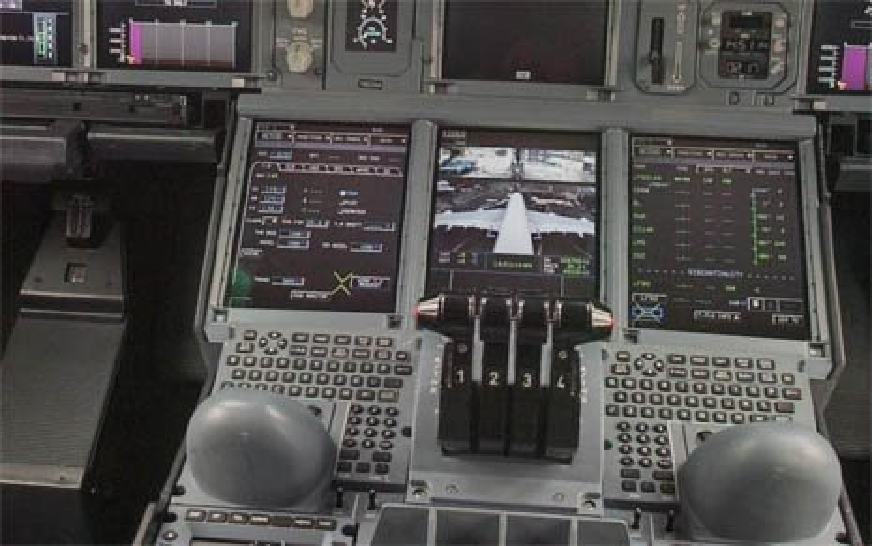
\includegraphics [scale = 0.5]{cockpit}
\end{center}
\caption{Dispositifs d'entrée et d'affichage à bord d'un cockpit}
\label{fig:cockpit} 
\end{figure}

La définition de  l'application interactive exprimée en  $L$ n'est pas
directement  exécutable, mais  elle  peut permettre,  en revanche,  de
générer  la structure  d'un code  exécutable pouvant  être celui  d'un
prototype  ou  de l'application  finale  destinée  à tourner  sur  une
plateforme donnée.  Différentes plateformes  et différents langages de
programmation peuvent être ciblés depuis  le langage abstrait $L$.  La
génération de code conforme à la norme ARINC 661 \cite{ARINC} offre un
exemple de  génération possible auquel  $L$ n'est pas limité  mais qui
concerne  directement  les   applications  aéronautiques  interactives
embarquées  à   bord  de  cockpits   tels  que  celui  de   la  figure
\ref{fig:cockpit}.

\subsection{Le contexte ARINC 661}

ARINC  661  est   la  norme,  utilisée  depuis   l'A380,  qui  définit
l'architecture  de   l'IHM  à  bord  des   cockpits  d'avions.   Cette
architecture répond, selon la norme, à une architecture client-serveur
et l'ARINC  661 définit donc  également le protocole  de communication
entre le  client et le  serveur qui,  tous deux, réalisent  le système
interagissant avec l'équipage à bord de l'avion.

Le serveur est  appellé le CDS (Cockpit Display  System).  Il comporte
les  dispositifs d'entrée  (clavier et  souris) et  de sortie  (écrans
LCD).  En se fondant sur une  bibliothèque de widgets dont il dispose,
le CDS intègre également dans  son noyau un gestionnaire d'événements,
d'affichage et  de widgets répartis  dans différentes fenêtres  que le
CDS gère également.  Il est ainsi responsable de la  création et de la
gestion  des  widgets,  de  la gestion  des  curseurs  graphiques,  de
l'affectation des entrées aux widgets  concernés et de la présentation
graphique de l'information.

\begin{figure}[tb!] 
\begin{center}
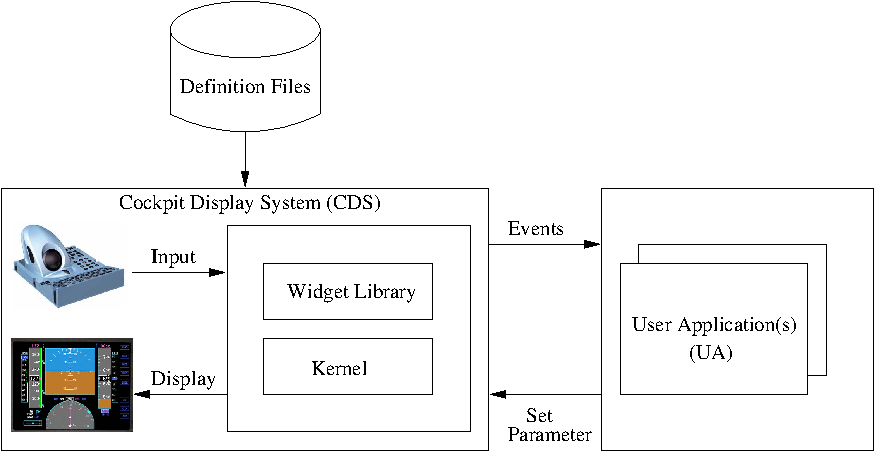
\includegraphics [scale = 0.52]{ARINC}
\end{center}
\caption{Architecture simplifiée de l'ARINC 661}
\label{fig:arinc} 
\end{figure}

La figure  \ref{fig:arinc}, qui  illustre l'architecture  proposée par
l'ARINC 661, montre en quoi le CDS  joue le rôle de serveur. Il reçoit
des  requêtes d'entrée  de l'équipage  et restitue,  en réponse  à ces
requêtes, des  informations d'affichage  sur les  écrans. Mais  le CDS
interagit également  avec ses clients  logiques que sont les  UA (User
Applications).  Ces  dernières sont  en prise  avec l'état  du système
piloté et  émettent à  destination du  CDS, par  le biais  de messages
\emph{Set  parameter},  des   requêtes  de  mise  à   jour  des  états
d'affichage de manière à ce que ce dernier présente à l'équipage toute
modification de l'état  de ce système. Elles reçoivent  en retour, par
le  biais de  messages  \emph{Event  Notification}, des  notifications
d'événements,  émis  par  les   widgets,  qui  reflètent  des  actions
possibles de l'équipage sur l'interface. Elles traitent ces événements
en envoyant, le cas échéant, des commandes au système piloté.

Le CDS, pour créer et gérer les  widgets, fait appel à des fichiers de
définition des IHM associées à chaque UA.  Ces fichiers définissent la
partie statique de  l'IHM qu'utilise une UA, comme  la disposition des
éléments sur l'écran, leurs couleurs, la fonte des textes \ldots 

Pour  des   raisons  de  sûreté,   les  interfaces  ARINC   sont  donc
relativement statiques.  Sauf  à l'initialisation, et sur  la base des
données fournies par les fichiers  de définition, il est impossible de
créer des  widgets ou de  les déplacer d'un  conteneur à l'autre  à la
volée lors de l'exécution. L'interface est définie de manière immuable
dans  le  CDS,   et  n'est  modifiable  à  l'exécution   que  via  les
modifications, opérées par les UA, de certains paramètres de contrôle.

La réalisation d'une IHM ARINC 661  consiste donc à créer deux entités
distinctes.  D'une part un fichier  de définition, hébergé par le CDS,
qui  définit  l'apparence  de  l'IHM  et  d'autre  part  l'application
utilisateur qui  en régit  le comportement. Le  langage $L$  permet de
décrire  avec précision  la partie  comportementale de  l'IHM sur  des
interacteurs abstraits. L'UA pourra donc être générée en grande partie
automatiquement à partir de sa définition en $L$.  Quand au fichier de
définition,  la  spécification  en   $L$  permet  d'en  construire  le
squelette  en permettant  de  construire  l'imbrication de  différents
contrôles dans  des conteneurs.  Mais, abstraite,  elle ne  permet pas
d'en  construire les  détails, comme  la  position et  la couleur  des
contrôles. Il faut donc concrétiser cette définition. 

\subsection{Concrétisation de la définition en $L$} 
\label{sec:concretisation}

Cette  concrétisation  consiste   pour  chaque  élément  d'interaction
abstrait,  à  choisir  le  type d'élément  d'interaction  concret  (le
widget)  disponible  qui  répond  le mieux  au  besoin.   Ainsi,  dans
l'application  présentée en  exemple,  certains  interacteurs de  type
\lstinline$NumericOutput$  sont  associés  à des  widgets  labels,  et
certains autres  à des  widgets jauges graphiques.   La concrétisation
consiste également à regler finement  les paramètres et l'apparence de
l'ensemble de  l'interface graphique. Elle se  base principalement sur
des critères ergonomiques,  et permet de se focaliser  sur les aspects
graphiques et visuels de l'interface.

\subsection{La génération de code ARINC 661}

La génération du  squelette de fichier de  définition est relativement
simple.  Une fois  les widgets  choisis et  associés aux  interacteurs
abstraits de la  définition $L$, une première  opération de génération
consiste à placer les éléments  d'IHM dans des conteneurs, imbriqués à
la manière  de l'arborescence des  interacteurs, et à leur  donner des
identifiants  uniques permettant  à l'application  utilisateur de  les
identifier.  Le  fichier  de   définition  ainsi  genéré  n'est  qu'un
squelette qui est ensuite complété lors de l'étape de concrétisation.

La  génération   du  code   de  l'application  utilisateur   est  plus
complexe. L'approche actuelle consiste dans un premier temps à aplanir
l'arborescence  des  interacteurs  et  à  reprendre  les  identifiants
définis lors de  la génération du squelette de  fichier de définition.
Un  premier  bloc  de  code   est  généré  à  partir  du  comportement
\lstinline$Init$ de chaque  interacteur.  Puis le bloc  de gestion des
évenements en provenance  du CDS est généré à partir  de la définition
des   comportements  de   chaque   interacteur.    A  chaque   section
\lstinline$When$ de  chaque instance d'interacteur correspond  un bloc
de code traitant l'évènement correspondant. Dès que le traitement d'un
évenement nécéssite  la modification d'une variable  impliquée dans la
section   \lstinline$Always$   d'un   interacteur,   les   traitements
nécéssaires  à   la  vérification  de  l'invariant   sont  ajoutés  au
traitement.

Lorsque la  définition abstraite en $L$  a été concrétisée et  que les
codes ont été  générés, l'application est prête à  être déployée. Dans
le context ARINC 661, cela revient  à charger le fichier de définition
sur le CDS,  le code de l'UA  sur son système cible, et  à exécuter le
tout.

\section{Conclusions et perspectives}
\label{sec:conclusion}


\small
\bibliographystyle{acm-sigchi}
\bibliography{bruno}


\end{document}
